\subsection{Overcoming Overconfidence and Capturing Physical Non-Identifiability}
\label{sec:non_identifiability}

A fundamental challenge in inverse problems for physiological systems is the inherent non-identifiability of parameters; multiple parameter configurations can yield identical observational data. An ideal probabilistic model must not only provide accurate point estimates but also reliably quantify this epistemic uncertainty by mapping the true solution manifold.

As shown in Figure \ref{fig:posterior_analysis}a, both the Single CVAE baseline and the proposed A-DCVAE appear to capture the global population distribution $p(\vtheta)$ reasonably well. This global coverage explains the competitive point-estimate metrics of the baseline model (Table \ref{tab:quantitative_results}), where the Single CVAE achieves nominally lower RMSE for both $S_I$ and $\sigma$. However, relying solely on standard regression metrics like RMSE in non-identifiable systems yields an ``illusion of accuracy.'' 

\begin{figure}[t]
    \centering
    \begin{subfigure}[b]{0.48\textwidth}
        \centering
        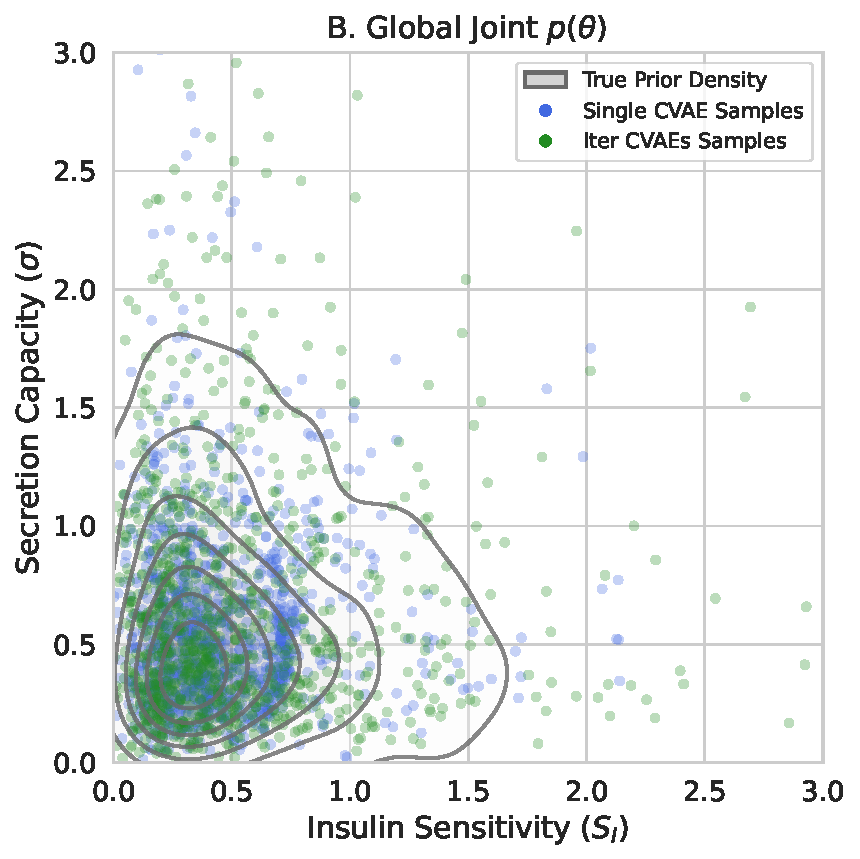
\includegraphics[width=\textwidth]{figures/figure3_B_global_2D.pdf}
        \caption{Global Joint $p(\vtheta)$}
        \label{fig:global_joint}
    \end{subfigure}
    \hfill
    \begin{subfigure}[b]{0.48\textwidth}
        \centering
        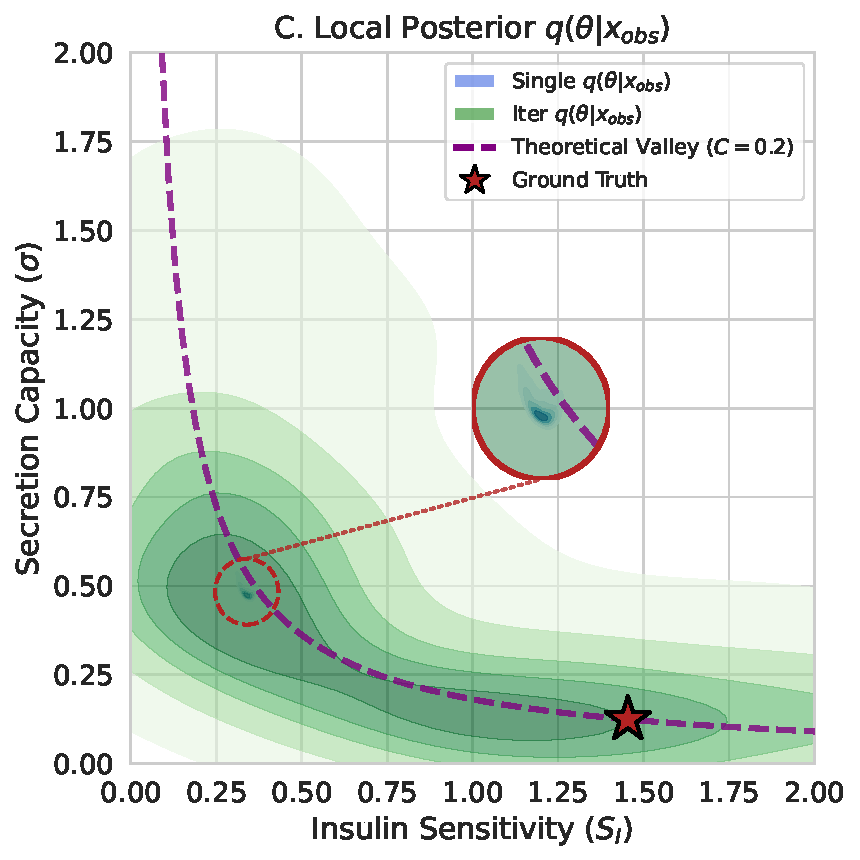
\includegraphics[width=\textwidth]{figures/figure3_C_local_2D.pdf}
        \caption{Local Posterior $q(\vtheta \mid \mX_{\mathrm{obs}})$}
        \label{fig:local_posterior}
    \end{subfigure}
    \caption{Visualizing the probabilistic capabilities of the models. (\textbf{a}) At the population level, both models adequately cover the global prior distribution. (\textbf{b}) At the individual sample level, the Single CVAE (blue) exhibits severe pathological mode collapse, predicting an extremely narrow distribution that misses the ground truth (red star). In contrast, A-DCVAE (green) accurately model the theoretical non-identifiability manifold ($S_I \times \sigma = C$, purple dashed line), providing well-calibrated posterior uncertainty.}
    % figure3_B/C regenerated with unified "A-DCVAE" legend via
    % prob_models/paper/experiments/regen_figure3.py (canonical checkpoints, seed 42).
    \label{fig:posterior_analysis}
\end{figure}

The critical failure of the baseline becomes evident when examining the local posterior $q(\vtheta \mid \mX_{\mathrm{obs}})$ for a specific observation. As illustrated in the inset of Figure \ref{fig:posterior_analysis}b, the Single CVAE suffers from pathological mode collapse. It exhibits extreme overconfidence, predicting a nearly point-like distribution (MPIW of 0.0102) that completely misses the true parameter. This phenomenon indicates that the baseline network merely memorizes a regression-to-the-mean mapping rather than understanding the underlying data generation mechanism. Consequently, this overconfidence results in a catastrophically poor Prediction Interval Coverage Probability (PICP) of 17.20\% and an exploding Negative Log-Likelihood (NLL) of 31990.99, rendering the model's probabilistic outputs practically useless for clinical or scientific inference.

\begin{table}[b]
    \centering
    \caption{Quantitative evaluation of parameter estimation and uncertainty calibration.}
    \label{tab:quantitative_results}
    \resizebox{\textwidth}{!}{
    \begin{tabular}{lcccccc}
        \toprule
        \multirow{2}{*}{\textbf{Model}} & \multicolumn{2}{c}{\textbf{Point Estimation}} & \multicolumn{4}{c}{\textbf{Probabilistic Calibration}} \\
        \cmidrule(lr){2-3} \cmidrule(lr){4-7}
        & \textbf{RMSE ($S_I \downarrow$ / $\sigma \downarrow$)} & \textbf{Pearson r ($S_I \uparrow$ / $\sigma \uparrow$)} & \textbf{PICP ($\uparrow$)} & \textbf{MPIW ($\downarrow$)} & \textbf{CRPS ($\downarrow$)} & \textbf{NLL ($\downarrow$)} \\
        \midrule
        Single CVAE & \textbf{0.1452} / \textbf{0.1480} & \textbf{0.8957} / \textbf{0.9371} & 17.20\% & \textbf{0.0102} & \textbf{0.0561} & 31990.99 \\
        A-DCVAE (Ours) & 0.1642 / 0.1811 & 0.8879 / 0.9311 & \textbf{99.44\%} & 1.1466 & 0.0836 & \textbf{-0.8076} \\
        \bottomrule
    \end{tabular}
    }
\end{table}

In stark contrast, the proposed A-DCVAE demonstrates a profound capacity to learn the physical laws governing the system. As shown in Figure \ref{fig:posterior_analysis}b, the generated posterior seamlessly stretches along the theoretical non-identifiability curve ($S_I \times \sigma = C$), successfully encompassing the ground truth within its predicted high-density region. By fully acknowledging the inherent uncertainty of the inverse problem, our approach achieves near-perfect calibration with a 99.44\% PICP and a highly stable negative NLL (-0.8076). These results demonstrate that while deterministic-like point estimation may yield marginally better RMSE, A-DCVAE provides a mathematically sound and physically valid probabilistic framework essential for reliable parameter inference.

\paragraph{Coverage versus sharpness, read honestly.}
The 99.44\% PICP is bought with a far wider mean interval (MPIW $0.0102 \to 1.1466$), which invites the objection that our posterior is merely under-confident. Two points sharpen the reading. First, the comparison is not width-for-width: the Single CVAE's narrow interval is \emph{false} confidence---it misses the truth (PICP 17.20\%), so its small MPIW measures precision about the wrong location. Second, and more importantly, under genuine non-identifiability a wide marginal is the \emph{correct} answer only if the width is spent along the unidentifiable direction and not across the identifiable one; aggregate MPIW cannot make this distinction, since it collapses a two-dimensional interval into a single scalar. The appropriate test is directional---whether the posterior stays tight across the identifiable combination ($mDI = S_I \times \sigma$) while extending along the non-identifiable fiber---which we assess directly against an analytic reference posterior next (\Secref{sec:reference}) and against strong baselines in \Secref{sec:baselines}. Judged by interval \emph{shape} relative to the fiber rather than by scalar width, A-DCVAE is faithful exactly where the single baseline is falsely confident.

\subsection{Validation against an analytic reference posterior}
\label{sec:reference}

Because glucose depends on $\vtheta$ only through the product $mDI = S_I\,\sigma$, the OGTT posterior admits a cheap gold standard: $p(S_I,\sigma \mid G) \propto \mathcal{L}(mDI)\,p(S_I,\sigma)$, evaluated on a grid by forward-simulation. This lets us grade the sampler against a reference rather than by self-consistency alone. Figure~\ref{fig:reference} overlays A-DCVAE's stationary samples $\pi^\ast$ on the reference density. Aggregated over eight observations, the reference confirms the identifiability structure numerically: its MAP $mDI$ is within $2.4\% \pm 2.0\%$ of the truth and its across-fiber coefficient of variation in $mDI$ is $10.0\% \pm 1.4\%$ (tight $\Rightarrow$ $mDI$ is identifiable), while the along-fiber extent is set by the prior. A-DCVAE follows the fiber \emph{direction} but is over-dispersed: its across-fiber $mDI$ CV is $80.5\% \pm 3.5\%$ against the reference's $10\%$, with a consistent offset (sliced-$W_2$ $0.20 \pm 0.14$; $W_1$ in $\log mDI$ $0.489 \pm 0.011$). We report this honestly as the visible approximation gap---the $\varepsilon_{\mathrm{app}}$/$\varepsilon_{\mathrm{inc}}$ of \Secref{subsec:theory} made concrete: the method recovers the correct one-dimensional support but not yet its exact width, an over-coverage rather than the baseline's catastrophic miss.

\begin{figure}[t]
    \centering
    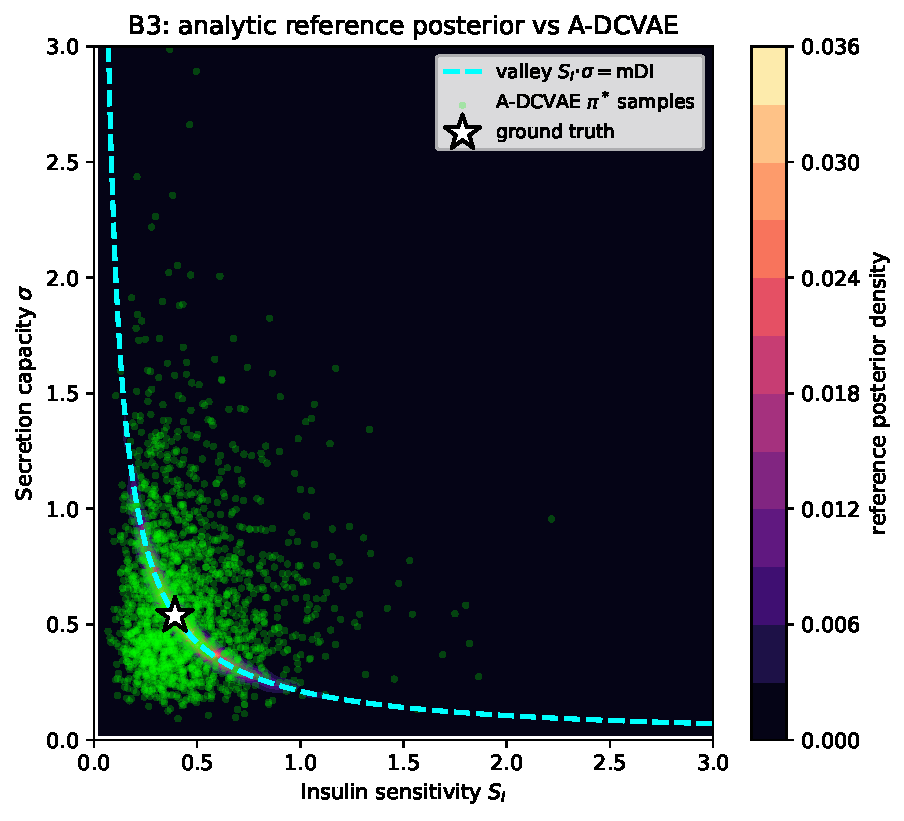
\includegraphics[width=0.62\textwidth]{figures/figure_b3_reference_posterior.pdf}
    \caption{\textbf{Analytic reference posterior vs.\ A-DCVAE.} The reference density $p(S_I,\sigma \mid G) \propto \mathcal{L}(mDI)\,p(S_I,\sigma)$ (color) is a thin crescent on the fiber $S_I\,\sigma = mDI$ (dashed). A-DCVAE's samples $\pi^\ast$ (green) follow the fiber direction through the ground truth (star) but are over-dispersed across it---the honest approximation gap.}
    \label{fig:reference}
\end{figure}

\subsection{Does decoupling help? A matched-budget baseline comparison}
\label{sec:baselines}

A natural worry is that decoupling into two conditionals buys nothing over directly modeling $p(\vtheta \mid \mX_{\mathrm{obs}})$ with a single expressive network. We test A-DCVAE against a self-contained conditional-flow NPE baseline (a single RealNVP over $p(\vtheta \mid \mX_{\mathrm{obs}})$) and a deterministic MSE regressor (a point estimator), all trained on an identical context (same data, split, and normalizer) per run and graded against the analytic reference ($5$ seeds $\times$ $5$ observations). Table~\ref{tab:baselines} and Figure~\ref{fig:baselines} report the canonical-scale ($50$k-simulation, patience-matched) result. A-DCVAE is closest to the reference in sliced-$W_2$ ($0.170$ vs.\ the flow's $0.533$) and competitive in direction ($mDI$ rel-err $0.016$ vs.\ $0.013$), while the deterministic regressor collapses (along-fiber std exactly $0$). The flow's much higher raw HPD-$95$ coverage ($0.57$ vs.\ $0.20$) is not accuracy but over-dispersion: its along-fiber spread ($2.10$) is roughly three times both the reference scale and A-DCVAE's ($0.71$).

\begin{table}[t]
    \centering
    \caption{Canonical-scale ($50$k, patience-matched) comparison against the analytic reference posterior, mean $\pm$ std over $5$ seeds $\times$ $5$ observations. Best in each column in bold.}
    \label{tab:baselines}
    \begin{tabular}{lcccc}
        \toprule
        \textbf{Method} & \textbf{ref-HPD95 cov.} & \textbf{along-fiber std} & \textbf{sliced-$W_2$ ($\downarrow$)} & \textbf{$mDI$ rel-err ($\downarrow$)} \\
        \midrule
        A-DCVAE (dual, ours) & $0.203 \pm 0.02$ & $0.712 \pm 0.01$ & $\mathbf{0.170 \pm 0.10}$ & $0.016 \pm 0.01$ \\
        NPE-flow (single RealNVP) & $0.572 \pm 0.06$ & $2.105 \pm 0.23$ & $0.533 \pm 0.07$ & $\mathbf{0.013 \pm 0.01}$ \\
        det-reg (point) & $1.000^{\dagger}$ & $0.000$ & $0.292 \pm 0.03$ & $0.020 \pm 0.01$ \\
        \bottomrule
    \end{tabular}
    \\[2pt]
    {\footnotesize $^{\dagger}$ A point estimate has a degenerate coverage of $1$ (or $0$); it carries no interval and is reported only for context.}
\end{table}

\begin{figure}[t]
    \centering
    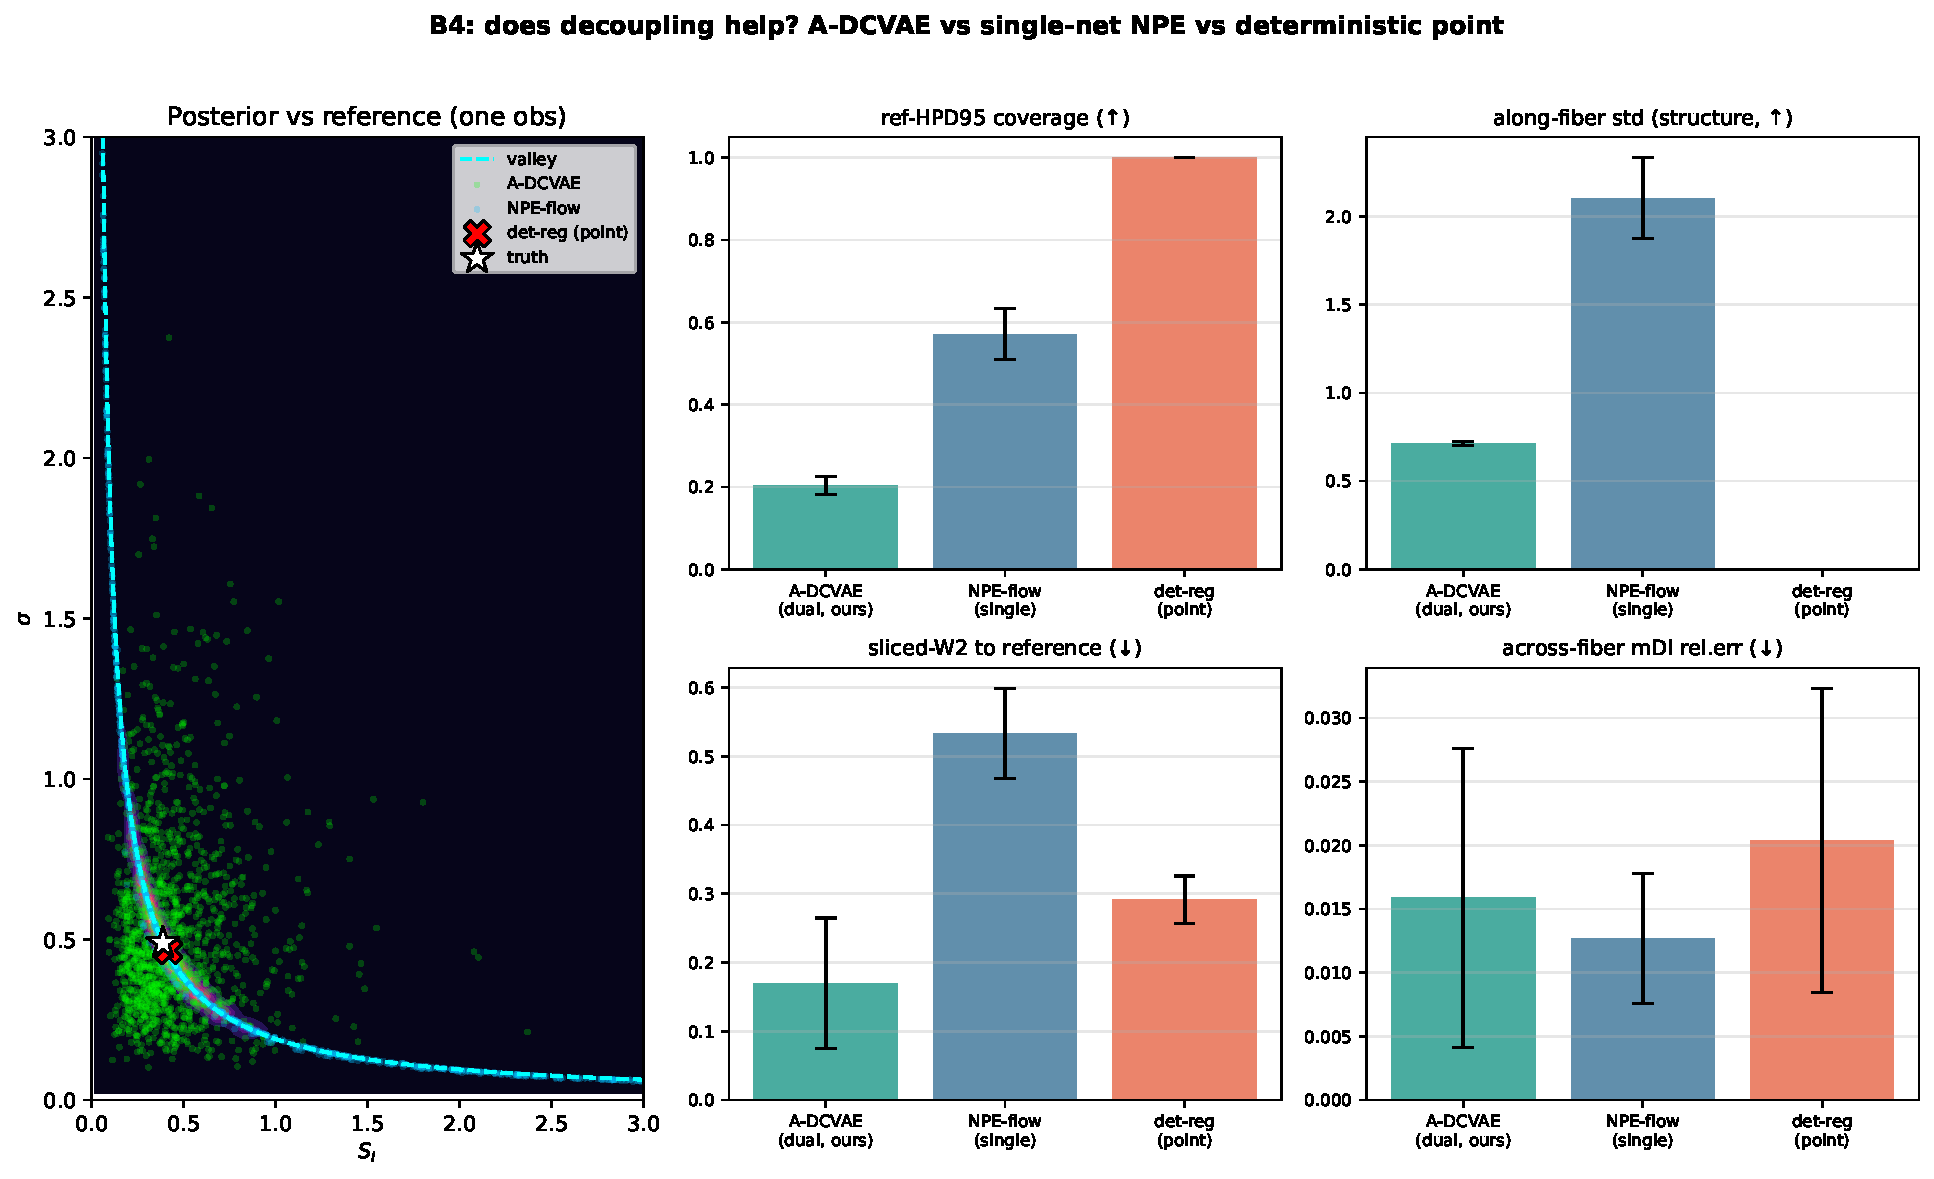
\includegraphics[width=\textwidth]{figures/figure_b4_baselines.pdf}
    \caption{\textbf{Does decoupling help?} (Left) posterior samples for one observation against the reference fiber; (right) the four metrics of Table~\ref{tab:baselines}. A-DCVAE (teal) is closest to the reference in sliced-$W_2$; NPE-flow (blue) is over-dispersed (high raw coverage, wide along-fiber spread); det-reg (red) collapses to a point.}
    \label{fig:baselines}
\end{figure}

We flag one honest caveat: at a smaller training scale ($10$k) the sliced-$W_2$ ordering reverses (flow $0.148$ vs.\ A-DCVAE $0.156$), so the accuracy advantage is scale-dependent, and we cite the canonical scale that matches our checkpoints. A patience-matched rerun rules out under-training as the explanation for the flow's canonical-scale gap: giving it five times more patience made it \emph{worse} (more over-dispersed), not better.

\subsection{Isolating the three guarantees}
\label{sec:ablation}

Finally, we isolate the three ingredients the theory assigns distinct roles (\Secref{subsec:theory}), ablating each noise source in turn over $5$ seeds at canonical scale (Figure~\ref{fig:ablation}). Removing \emph{condition} noise (N1) raises the empirical contraction constant from $\kappa = 0.41$ to $0.71$, toward the stability limit $\kappa = 1$---the predicted loss of the Jacobian/Tikhonov control; chain divergence stays zero (the state space is bounded), so the effect is on mixing \emph{rate}, not blow-up. Replacing the stochastic kernels with their deterministic mean maps (N4 off) collapses the along-fiber spread from $0.72$ to $0.000$ for the full model---regression-to-the-mean, reproduced on demand---confirming that injection noise is what averts collapse. Consistent with our own altitude assessment, \emph{target} noise (N2) shows no isolated benefit here (across-fiber $mDI$ error $\approx$ full), matching its status as a background principle rather than a load-bearing guarantee. The self-consistency certificate $\varepsilon_{\mathrm{inc}}$ stays ${\approx}0.03$ across variants, indicating $\pi^\ast$ is near self-consistent. One richer detail at canonical scale: when $\kappa$ is far from zero (N1 off), even the deterministic mean-map ping-pong no longer fully collapses (spread $0 \to 1.72$) within the step budget, reinforcing that the contraction knob (N1) and the non-collapse knob (N4) are genuinely separate.

\begin{figure}[t]
    \centering
    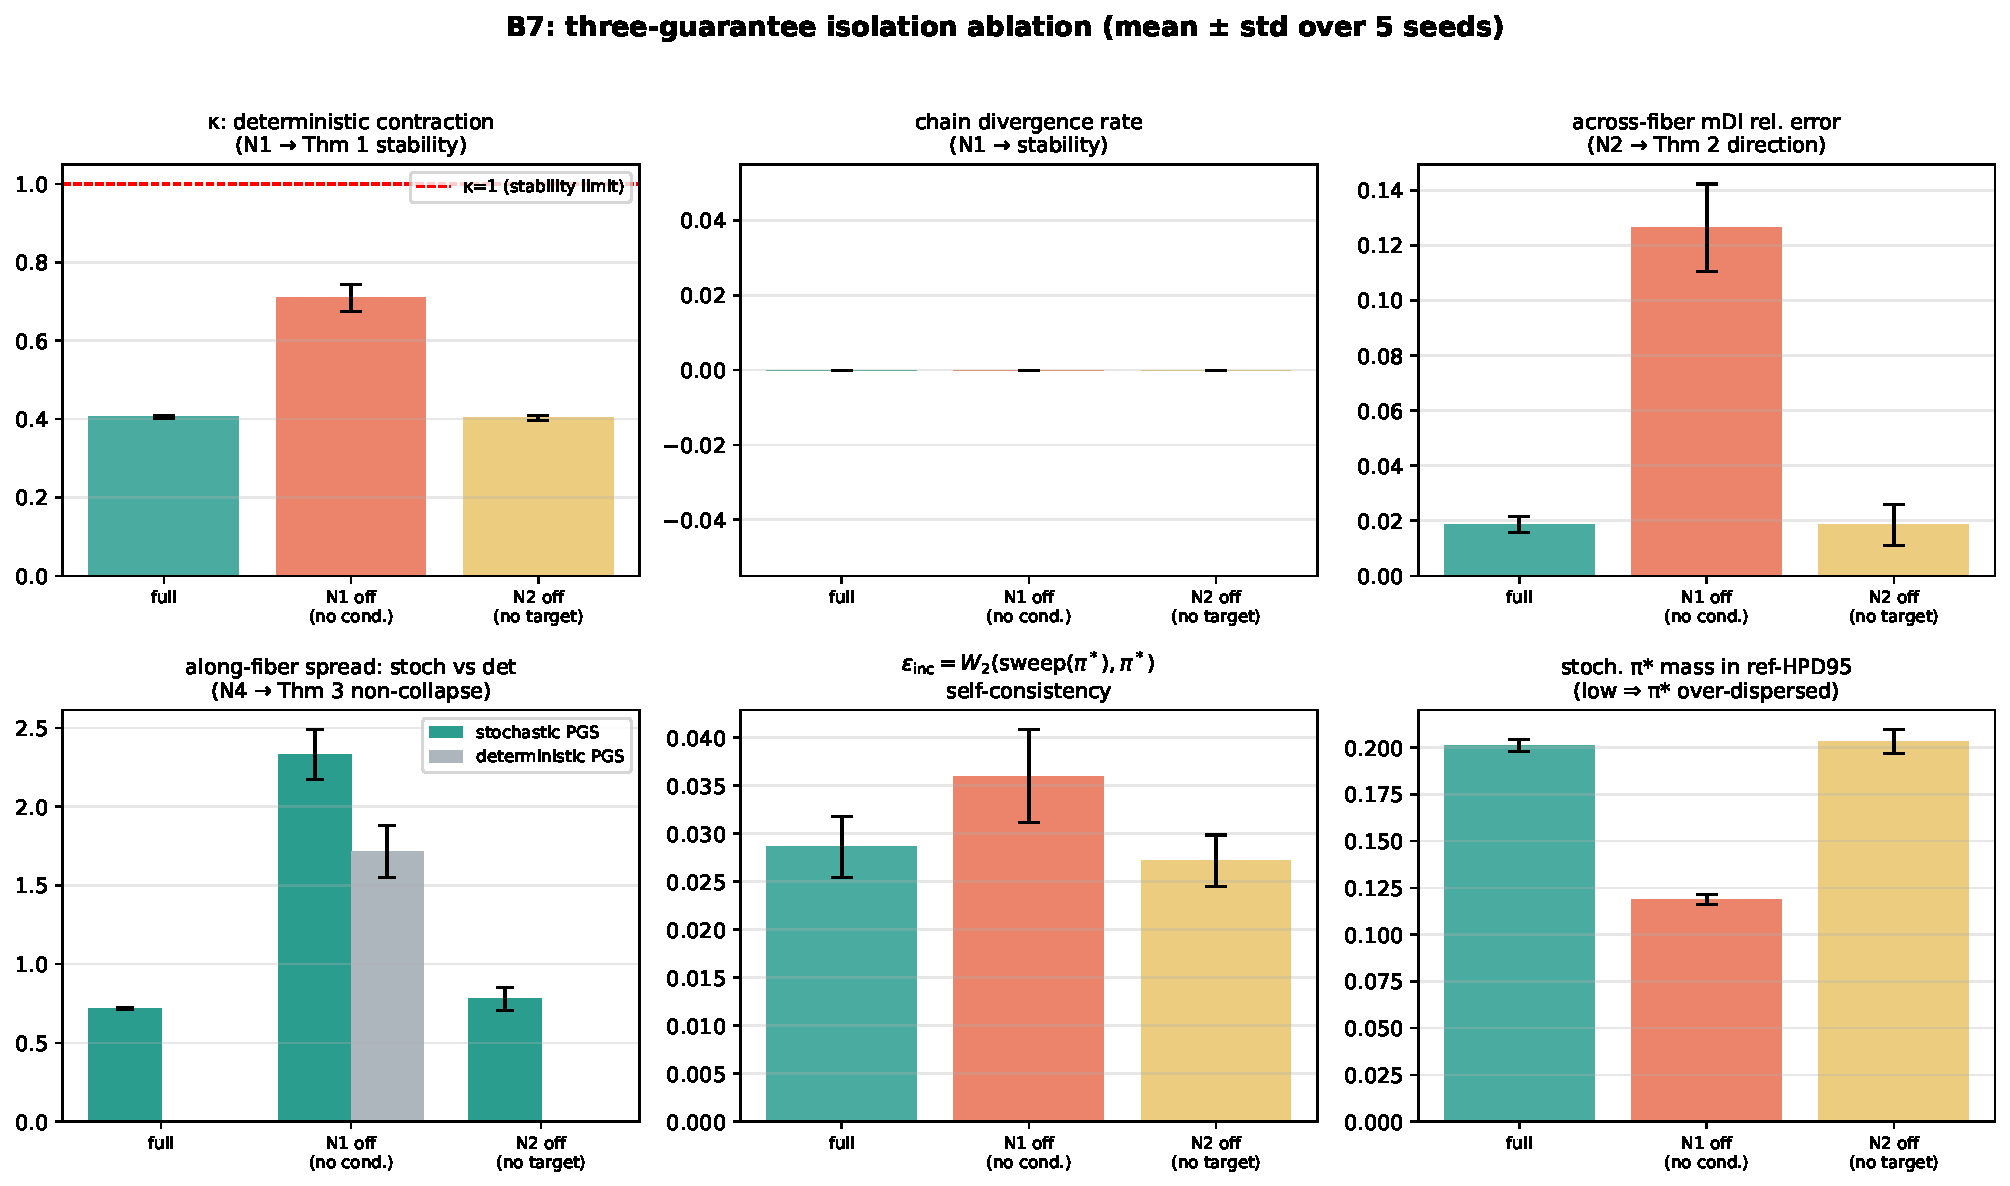
\includegraphics[width=\textwidth]{figures/figure_b7_ablation.pdf}
    \caption{\textbf{Three-guarantee isolation ablation} (mean $\pm$ std, $5$ seeds, canonical scale). Left to right, top then bottom: contraction $\kappa$ and chain divergence (N1 / stability), across-fiber $mDI$ error (N2 / direction), along-fiber spread stochastic vs.\ deterministic (N4 / non-collapse), self-consistency $\varepsilon_{\mathrm{inc}}$, and $\pi^\ast$ mass in the reference HPD-$95$. Removing condition noise raises $\kappa$; removing injection noise collapses the along-fiber spread to zero.}
    \label{fig:ablation}
\end{figure}